\section{Proposed approach}
\label{sec:apprach}

Given a set of existing DSLs (that we term as the \textit{input set}) our approach is intended to identify commonalities --and so, potential reuse--. Then, we provide some metrics that permit to objectively evaluate those commonalities. The reminder of this section explain how we tackle this problem.

\subsection{Identifying commonalities}
\label{sec:metrics}

In the first part of our approach, we perform static analysis in syntax and semantics of a given set of DSLs in order to build a pair of Venn diagrams that allows language designers to easily visually identify commonalities among DSLs under study. The idea is to visualize each DSL as a pair of two sets: The first one is a set of metaclasses representing the syntax, and the second one is a set of domain-specific actions representing the semantics. Syntactic and semantic commonalities are represented as intersections between the corresponding sets. To this end, we designed an algorithm that is able to compute the all intersections among the syntax of the DSLs in the input set. 

Our algorithm for detecting \textbf{syntactic intersections} can be described as by the function that receives a set of metamodels (one for each DSL of the input set) and returns a set of tuples containing all the intersections among these metamodels. Note that there can be intersections among any of the combinations of the input set. Hence, in the result there is a tuple for each of the possible combinations of the input metamodels (i.e., the power set). Similarly, our algorithm for detecting \textbf{semantic intersections} can be described as a function that receives a set of aspects (one for each DSL of the input set) and returns a set of tuples containing all the intersections among these aspects. Figure \ref{fig:shape} shows the Venn Diagram for the case of our motivating scenario. In that figure we can see that the family is an overlapping family in terms of the abstract syntax. 

\begin{figure}
\centering
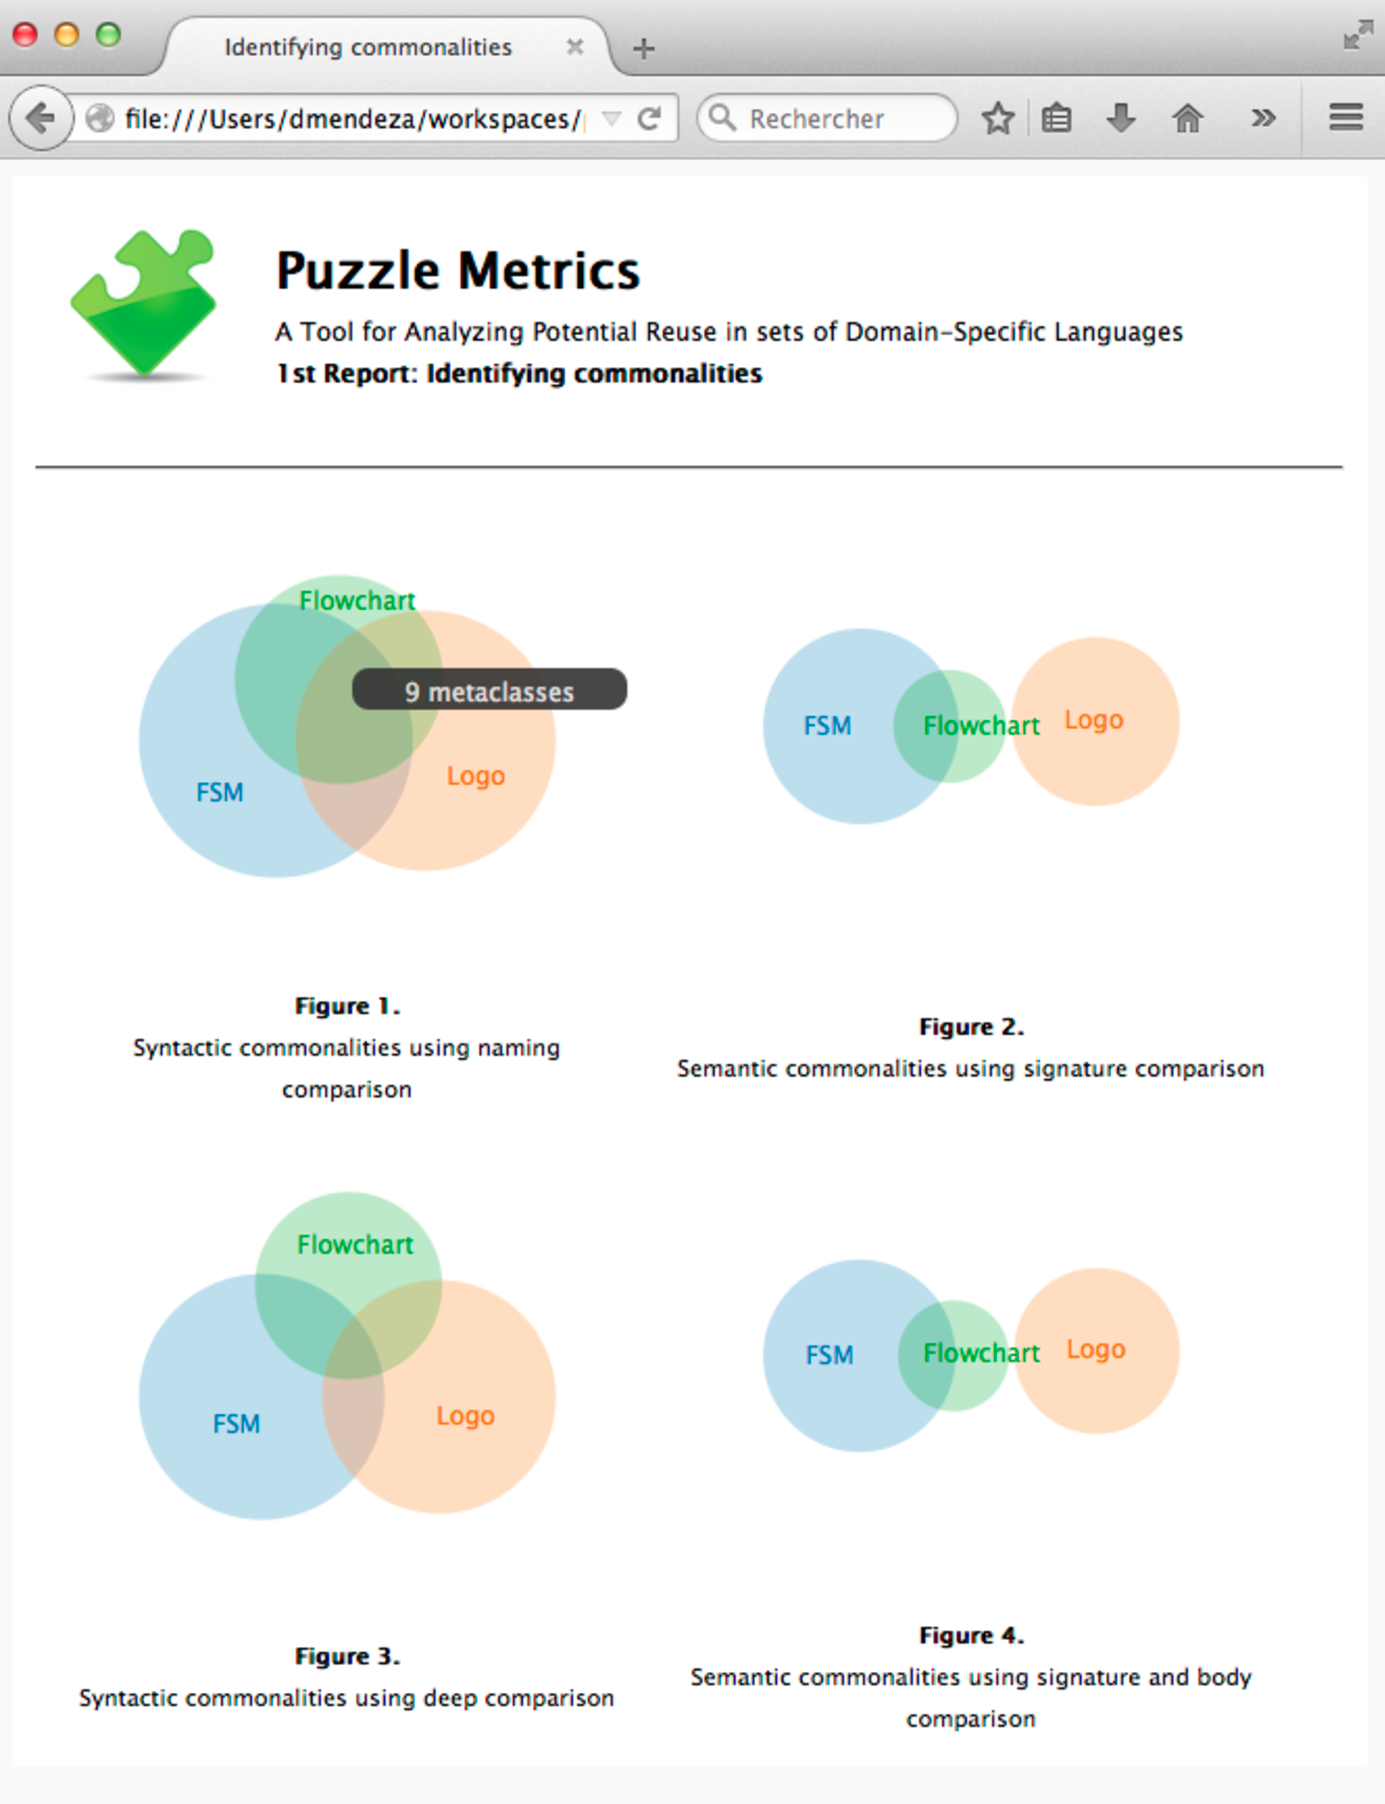
\includegraphics[width=1\linewidth]{images/domains-inaction.pdf}
\caption{Visualizing syntactic and semantic commonalities}
\label{fig:shape}
\end{figure}

\subsection{Measuring potential reuse}

As a second part of our analysis, we propose a quantitative evaluation of the potential reuse represented as commonalities in a set of DSLs. Such evaluation is based on the metrics introduced in \cite{Berger:2014} which are originally defined for software products in general and that we adapted for the case where the software products are domain-specific languages. We choose these metrics because they perfectly fit in the idea of conceiving potential reuse as intersections of Venn diagrams and because they were already evaluated in an industrial case study \cite{Berger:126283}.

\begin{figure}
\centering
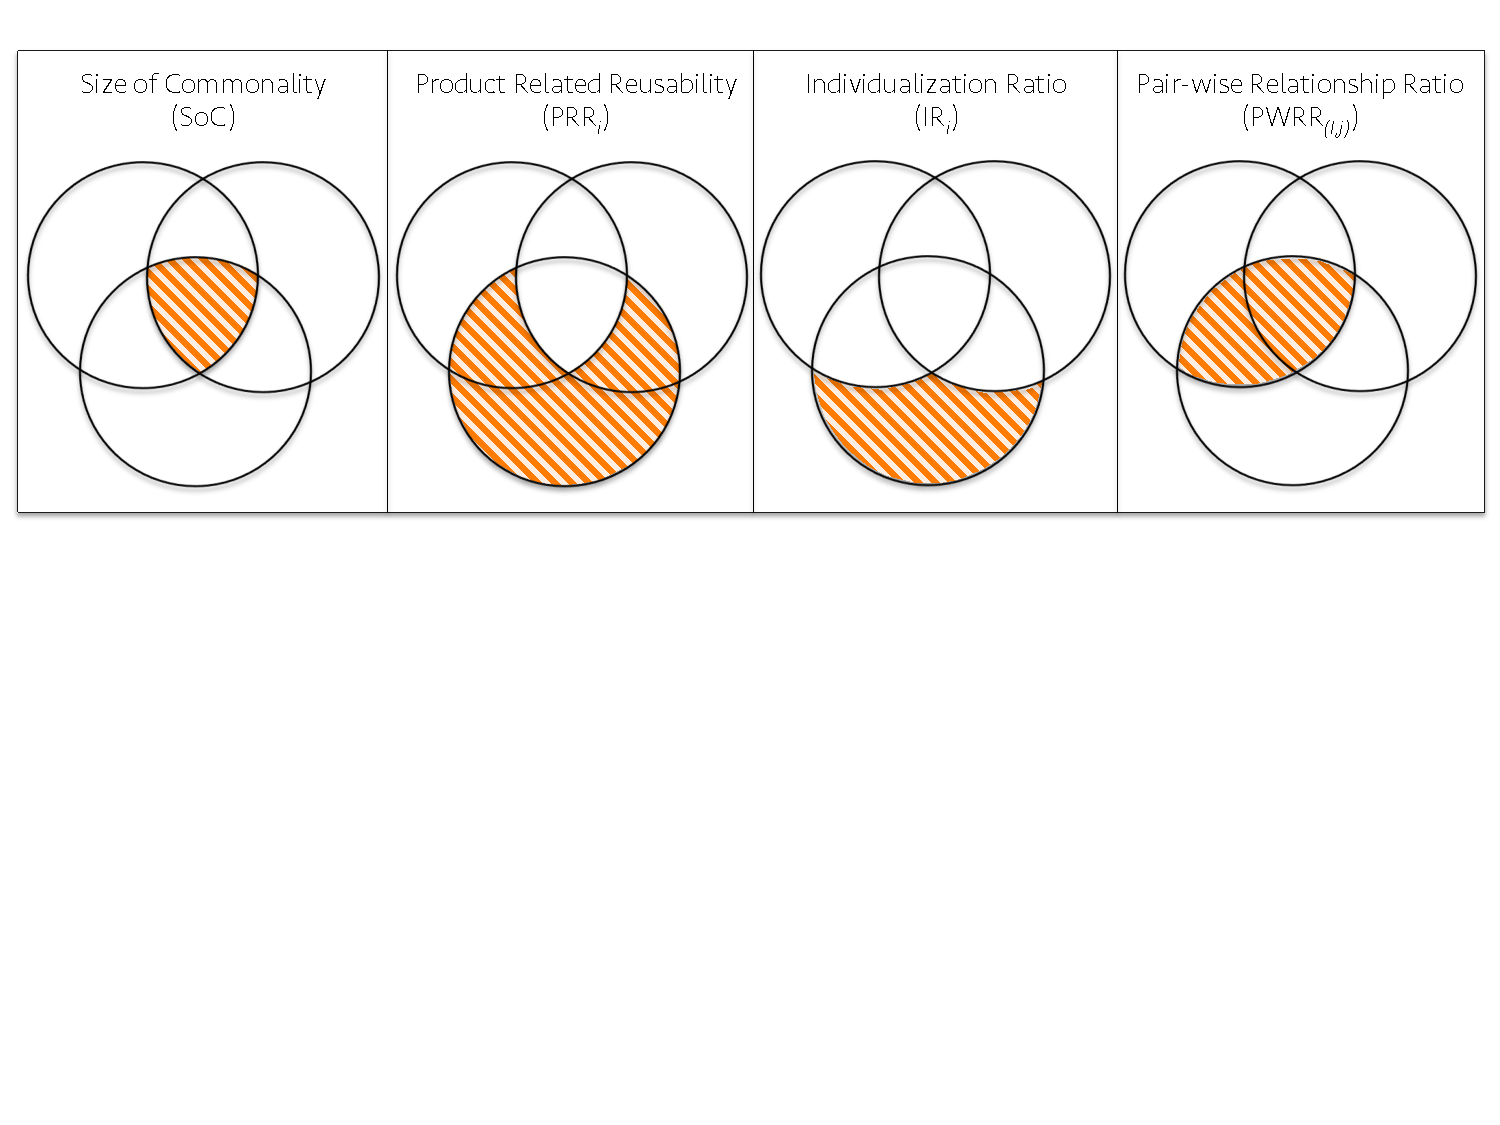
\includegraphics[width=1\linewidth]{images/metrics.pdf}
\caption{Metrics for evaluation of potential reuse}
\label{fig:metrics}
\end{figure}

Figure \ref{fig:metrics} shows the reuse metrics graphically. They are intended to normalize the size of the commonalities existing among the DSLs of the input set. To do so, the idea is to see the intersections in terms of percentages. Hence, they answer questions such as: what is the percentage of language constructs of a given DSL that are also defined in another DSL in the input set? In this section we present these metrics in terms of the formulas we used to compute them. It is important to remember that the results provided by those metrics also depend on the comparison operator.

\begin{itemize}
\item \textbf{Size of Commonality (SoC):} The size of commonality metric is intended to measure the amount of metaclasses and domain-specific actions that are shared by all the DSLs in the input set. It is defined as the size of the intersection of all the DSLs in the input set. 

\hspace{3mm} The usefulness of this metric relies on the identification of a common \textit{core} among all the DSLs. This is quite relevant because there are certain reuse approaches for DSLs (such as the one presented in \cite{Zschaler:2010b}) where the existence of a core is a prerequisite.

%\begin{equation}
%  SoC_{syn}(dsls) = |\bigcap _{i=0}^{|dsls|}dsls_i.syn|
%\end{equation}
%\vspace{-1mm}
%\begin{equation}
%  SoC_{sem}(dsls) = |\bigcap _{i=0}^{|dsls|}dsls_i.sem|
%\end{equation}

\vspace{1mm}
\item \textbf{Product-Related Reusability ($PRR_i$):} The product-related reusability is a metric that, for each DSL of the input set, measures the percentage of the metaclasses and domain-specific actions that are defined in the core detected by the SoC metric. It permits to see how related is each DSL with the core of the input set.

%\begin{equation}
%  PRR_{syn}(dsls,i) = \frac{|dsls_i.syn|}{SoC_{syn}(dsls)} \times 100\% 
%\end{equation}
%\vspace{-1mm}
%\begin{equation}
%  PRR_{sem}(dsls,i) = \frac{|dsls_i.sem|}{SoC_{sem}(dsls)} \times 100\% 
%\end{equation}

\vspace{2mm}
\item \textbf{Individualization Ratio ($IR_i$):} The individualization ratio is a metric that, for each DSL in the input set, measures the percentage of the metaclasses and domain-specific actions that are common with at least another DSL. This metric shows how particular is each language. That is, how many metaclasses and domain-specific actions are tailor-made for the DSL. 

%\begin{equation}
%  IR{syn}(dsls,i) = \frac{|dsls_i.syn|}{|\{x \mid (\exists d \in dsls \mid d \neq dsl_i \wedge x \in d.syn)\}|} \times 100\%
%\end{equation}
%\vspace{-1mm}
%\begin{equation}
%  IR{sem}(dsls,i) = \frac{|dsls_i.sem|}{|\{x \mid (\exists d \in dsls \mid d \neq dsl_i \wedge x \in d.sem)\}|} \times 100\%
%\end{equation}

\vspace{2mm}
\item \textbf{Pairwise Relationship Ratio ($PWRR_{(i,j)}$):} The pair-wise relationship ration is a metric that measures the reusability between each possible pair of DSLs in the input set. This metric can be seen as a pair-wise similarity that indicates how different is a DSL for each of the other DSLs in the input set.

%\begin{equation}
%  PWRR_{syn}(i,j) = \frac{|dsls_i.syn|}{|dsls_i.syn| - |dsls_i.syn \cap dsls_j.syn|} \times 100\%
%\end{equation}
%\vspace{-1mm}
%\begin{equation}
%  PWRR_{sem}(i,j) = \frac{|dsls_i.sem|}{|dsls_i.sem| - |dsls_i.sem \cap dsls_j.sem|} \times 100\%
%\end{equation}
\end{itemize}
